%~~~~~~~~~~~~~~~~~~~~~~~~~~~~~~~~~~~~~~~~~~~~~~~~~~~~~~~~~~~~~~~~~~~~~
%    File      : webanalysis
%~~~~~~~~~~~~~~~~~~~~~~~~~~~~~~~~~~~~~~~~~~~~~~~~~~~~~~~~~~~~~~~~~~~~~

\textual
\newpage
%\chapter{Dependability}\label{cap:dependability}

\section{Sequence Diagrams}

In questa sezione vengono mostrati e commentati i sequence diagrams realizzati per le funzionalità più significative dell'applicazione realizzata.

\subsection{Scenario Login}

In figura \ref{gfx:sdlogin} è riportato lo scenario di Login, con le operazioni che il sistema effettua rispetto agli input inseriti dall'utente. Si nota che sulla base della risposta ricevuta dalla servlet viene visualizzato un differente messaggio di errore 

\begin{figure}[!htbp]
	\centering
	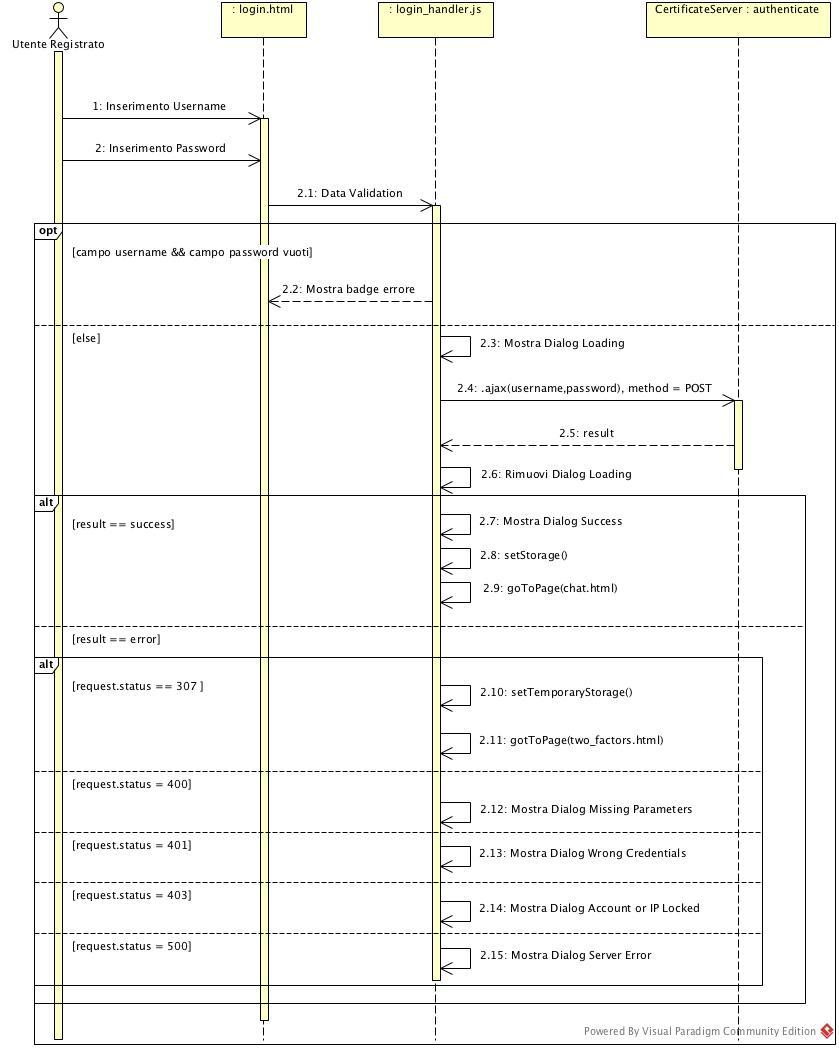
\includegraphics[scale = .4]{img/sd_login.jpg}
	\caption{Scenario Login}
	\label{gfx:sdlogin}
\end{figure}

\subsection{Scenario Registrazione}

In figura \ref{gfx:sdregister} è riportato lo scenario di Registrazione per gli utenti, con le operazioni che il sistema effettua rispetto agli input inseriti dall'utente, verificanti la validità della password in termini di strongness, richiedendo un carattere maiuscolo, uno minuscolo e un numero per un totale di almeno 8 caratteri, e dell'email, rispetto al formato. Si nota che sulla base della risposta ricevuta dalla servlet viene visualizzato un differente messaggio di errore.

\begin{figure}[!htbp]
	\centering
	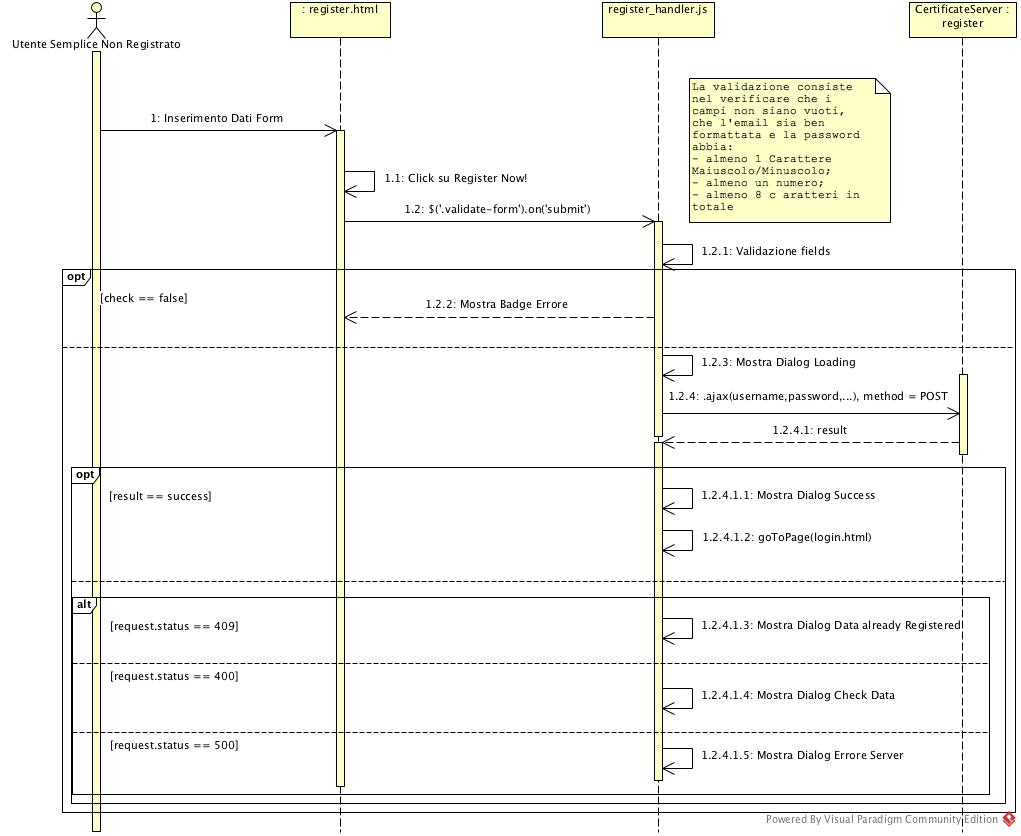
\includegraphics[scale = .4]{img/sd_register.jpg}
	\caption{Scenario Register}
	\label{gfx:sdregister}
\end{figure}

\subsection{Server Interaction (Login)}

In figura \ref{gfx:serverinteractionlogin} viene riportato il sequence diagram che descrive l'interazione che avviene tra il server NodeJS e il server Tomcat all'atto del login.

\begin{landscape}
\begin{center}

\begin{figure}[!htbp]
	\centering
	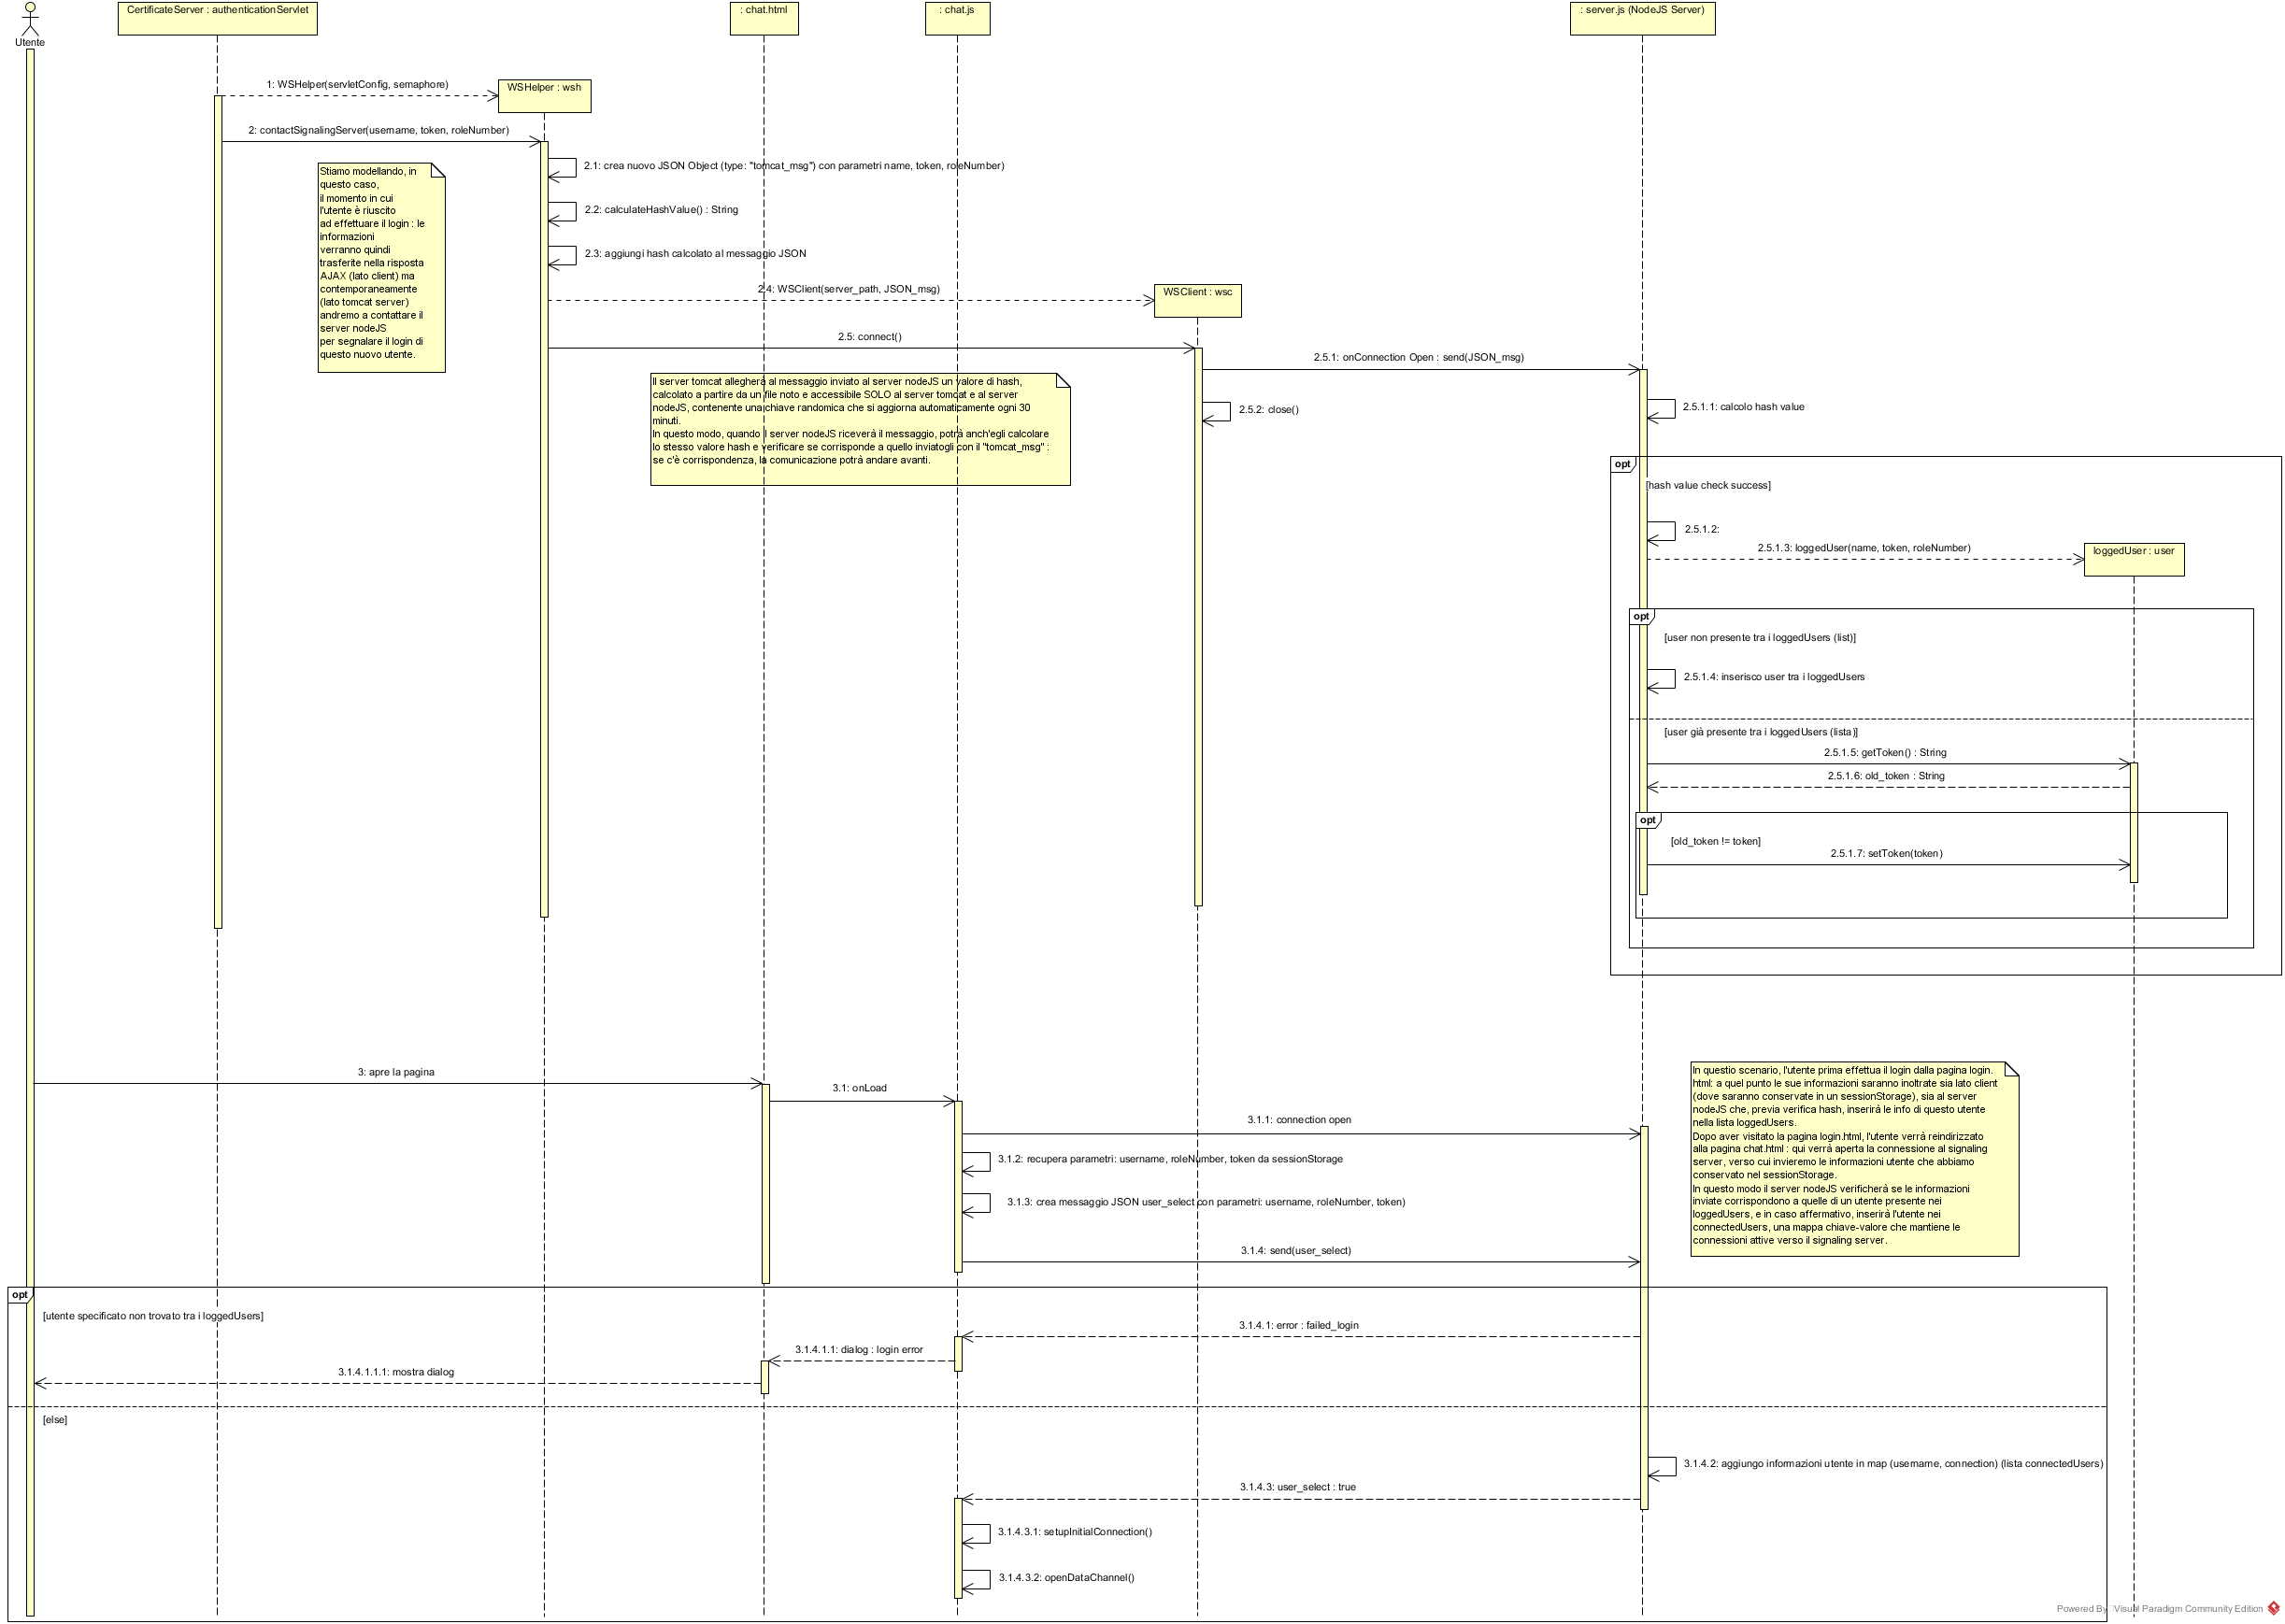
\includegraphics[scale = .31]{img/sequence_serverint.png}
	\caption{Server Interaction (Login)}
	\label{gfx:serverinteractionlogin}
\end{figure}
\end{center}	
\end{landscape}%

Quando un nuovo utente effettua correttamente il login presso la pagina login.html, accadono due cose:
\begin{itemize}
\item Le informazioni relative all'utente loggato vengono trasferite (come AJAX response) al client, che le conserva in un sessionStorage;
\item Il server Tomcat si occupa di contattare, mediante websocket, il server di segnalamento (nodeJS) per notificare il login di un nuovo utente.
\end{itemize}

Nel nostro caso, siamo interessati a modellare il secondo scenario.\\
Quando questo accade infatti, il server Tomcat aprirà una websocket verso il server nodeJS, passandogli le informazioni relative al nuovo utente loggato e, in aggiunta, un valore di hash: questo valore viene calcolato a partire da un file noto \textbf{esclusivamente} al server Tomcat e al server nodeJS (contenente una chiave randomica generata ogni 30 minuti): in questo modo, nel momento in cui il server nodeJS riceverà le informazioni sul login effettuato, potrà calcolare l'hash a partire dallo stesso file e verificarne la validità.\\
In caso di corrispondenza, il server nodeJS si occuperà di inserire l'utente specificato tra i cosiddetti \textit{loggedUsers}, ovvero coloro che hanno correttamente eseguito la procedura di login presso il server principale.\\
In questo modo, evitiamo che un qualsiasi utente possa contattare il server nodeJS e spacciarsi per un utente loggato.\\
Quando poi l'utente, accedendo alla pagina chat.html, si connetterà al signaling server (aprendo una websocket verso di esso), comunicherà a quest'ultimo le informazioni che ha ottenuto in fase di login (conservate nel sessionStorage) in modo che il server nodeJS potrà verificare se queste informazioni corrispondono effettivamente ad un utente presente tra i \textit{loggedUsers} (loggato correttamente): in caso affermativo, l'utente sarà inserito nei \textit{connectedUsers}, ovvero gli utenti con una connessione attiva verso il signaling server.\\
Per ulteriori dettagli si rimanda alla documentazione interna del server nodeJS.\\



\subsection{Offer Interaction}

In figura \ref{gfx:offerinteraction} si mostra l'interazione che si viene a realizzare ogniqualvolta un utente decide di inviare una \textit{offer} verso un altro utente, con l'intenzione di configurare e avviare una chat.

\begin{landscape}
\begin{center}
\begin{figure}[!htbp]
	\centering
	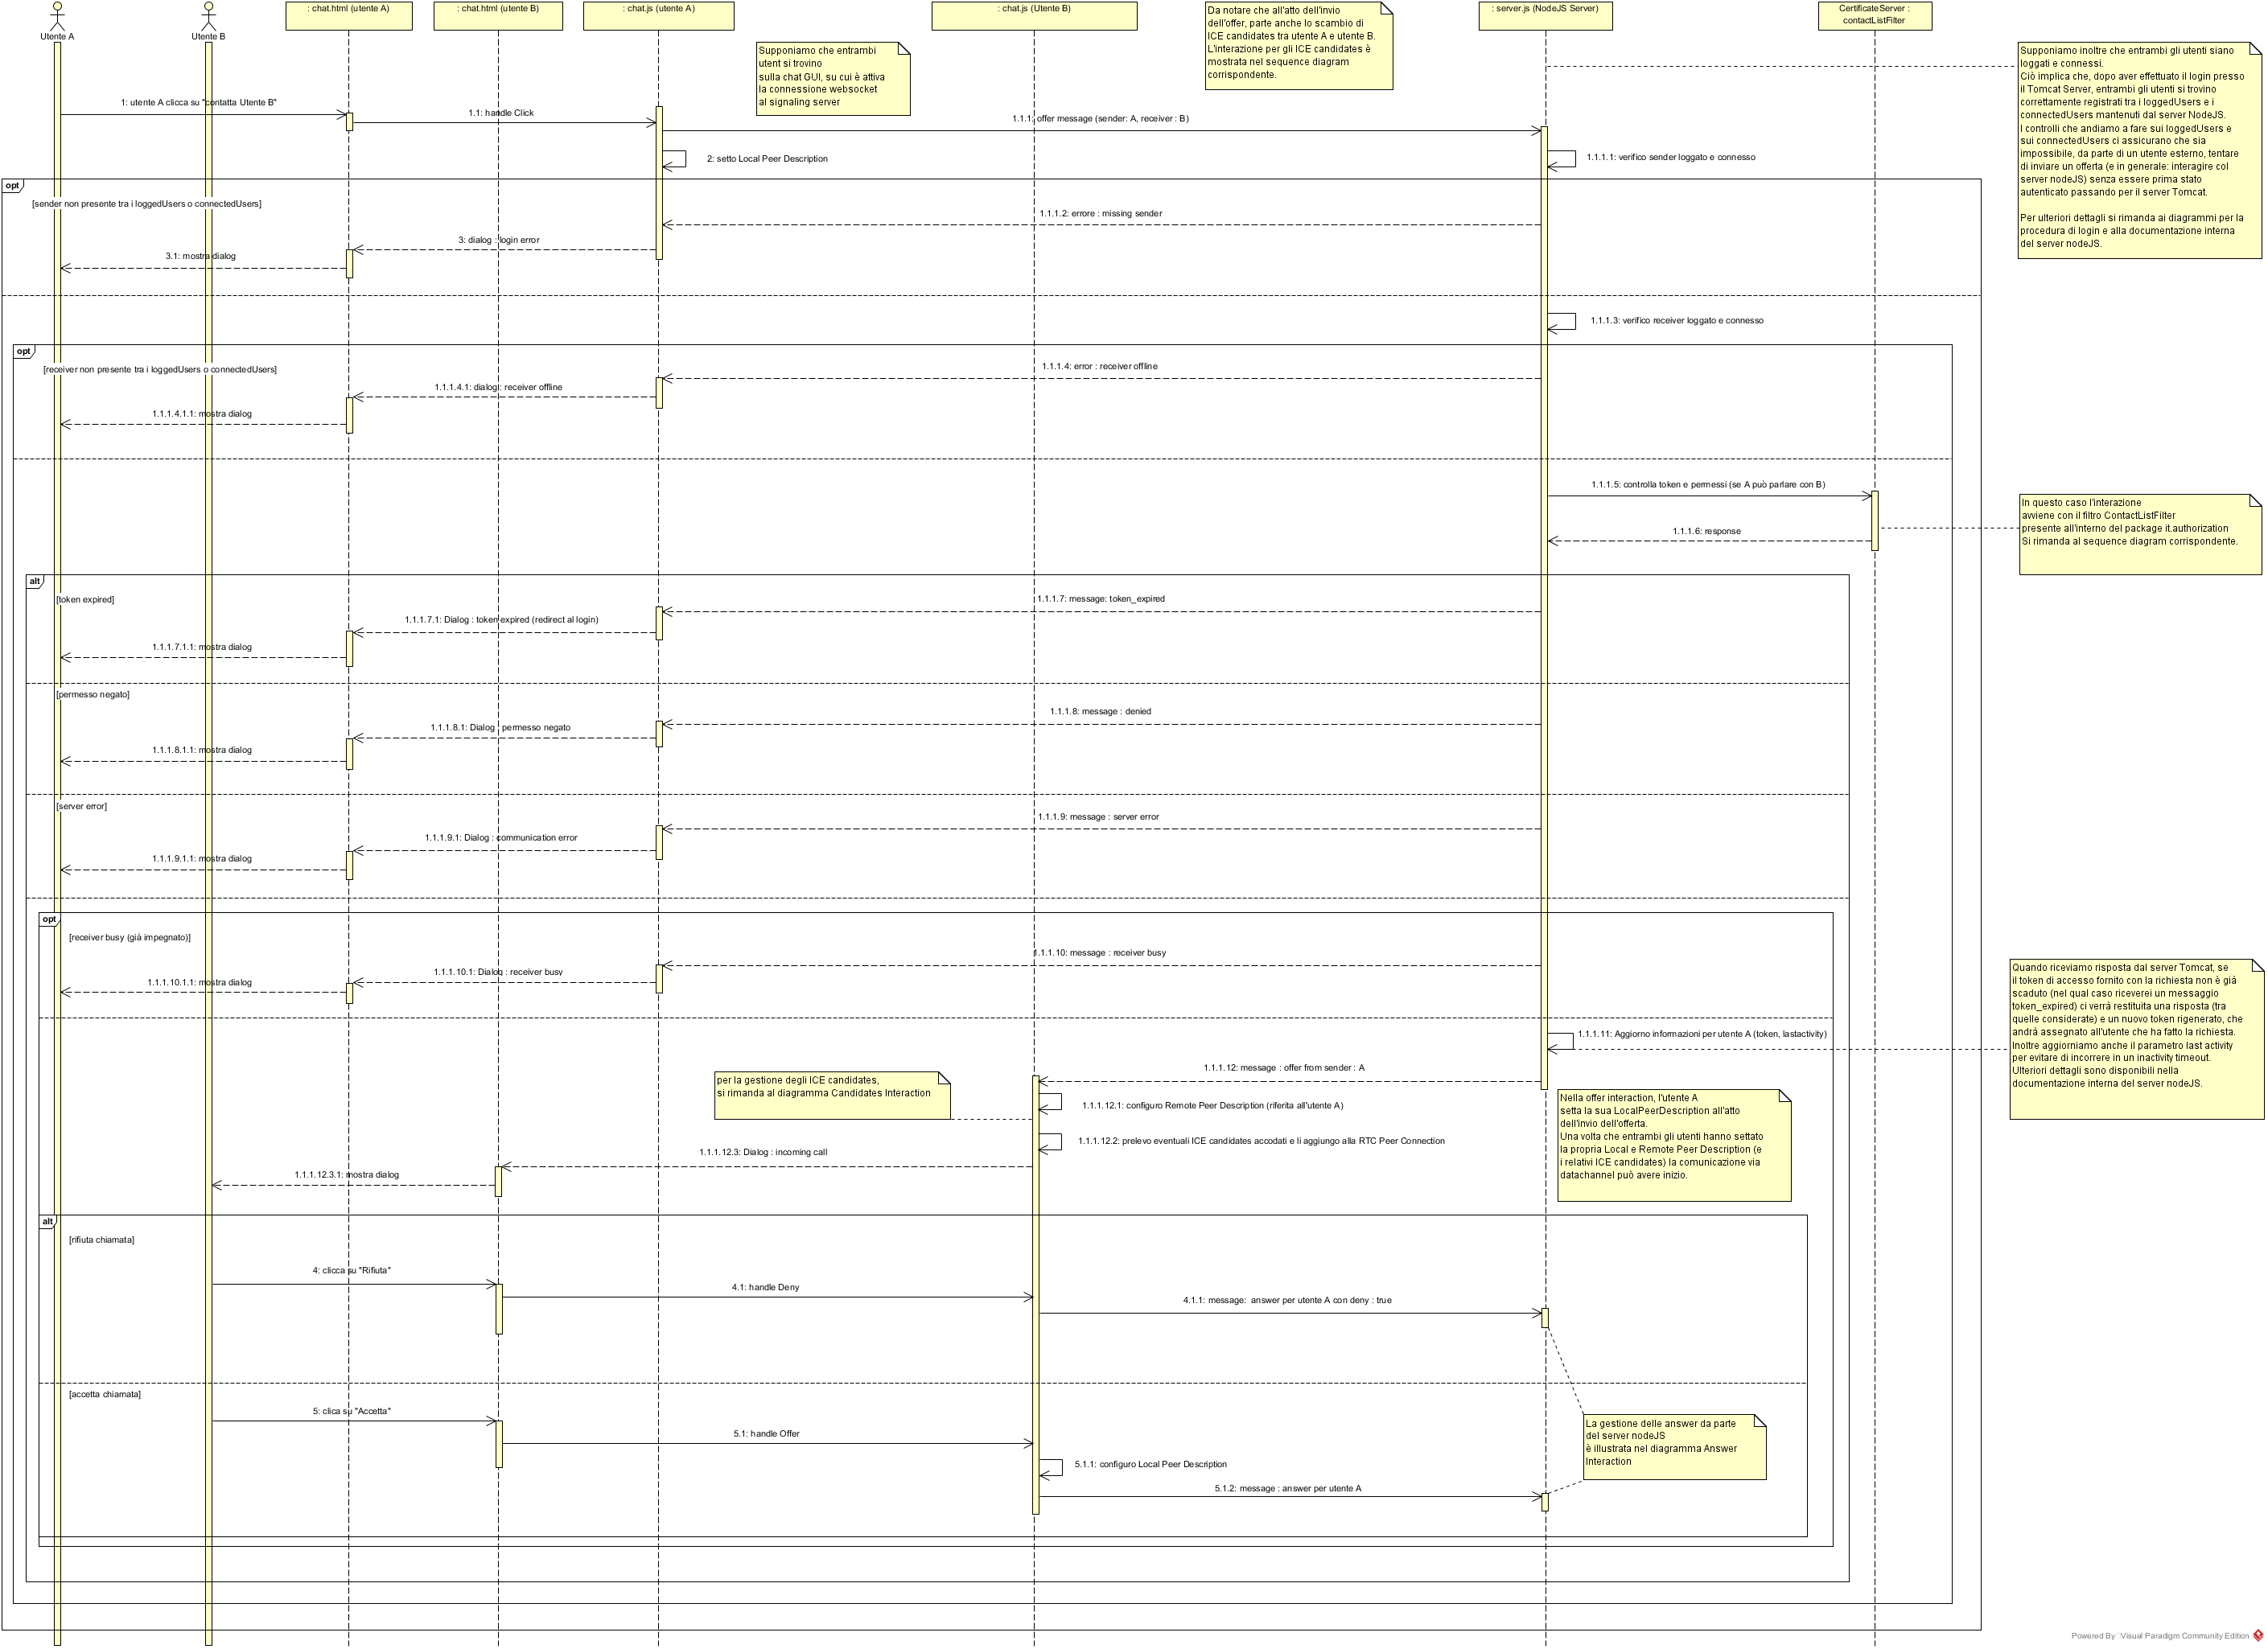
\includegraphics[scale = .25]{img/sequence_offer.png}
	\caption{Offer Interaction}
	\label{gfx:offerinteraction}
\end{figure}
\end{center}	
\end{landscape}%
Se supponiamo di avere un utente A che invia un messaggio offer destinato all'utente B, allora il server nodeJS, alla ricezione di tale messaggio, si occuperà di:
\begin{itemize}
\item verificare che l'utente A sia loggato e connesso (ovvero: presente tra loggedUsers e connectedUsers);
\item verificare che l'utente B sia loggato e connesso (ovvero: presente tra loggedUsers e connectedUsers);
\item verificare che l'access token di A sia valido;
\item verificare che A abbia il permesso di parlare con B (contattando il server tomcat e usando policy XACML);
\item verificare che B non sia già impegnato in un'altra chat.
\end{itemize}

Quando una di queste condizioni non dovesse essere verificata, il server nodeJS si occuperà di contattare il mittente (utente A) con un messaggio di stato opportuno.\\
Inoltre, se tutte le verifiche di cui sopra vanno a buon fine, il server nodeJS si occuperà di recapitare un messaggio offer verso l'utente B, che permetterà a quest'ultimo di configurare la comunicazione con l'utente A: in particolare, l'utente B potrà in questo modo configurare la sua \textit{LocalPeerDescription} (locale) e la \textit{RemotePeerDescription} (legata all'utente A, e ottenuta con le informazioni contenute nella offer).\\
Per ulteriori dettagli si rimanda alla documentazione interna del server nodeJS.\\


\subsection{Answer Interaction}

In figura \ref{gfx:answerinteraction} si riporta il sequence diagram che mostra l'interazione tra utente A e utente B nel momento in cui vi è l'invio di una \textit{answer}: supponendo che l'utente A voglia chiamare l'utente B, e che l'invio dell'offer sia avvenuto correttamente verso l'utente B, andremo a descrivere la comunicazione che avviene nel momento in cui B decide di inviare una answer ad A, tramite il signaling server.

\begin{landscape}
\begin{center}
\begin{figure}[!htbp]
	\centering
	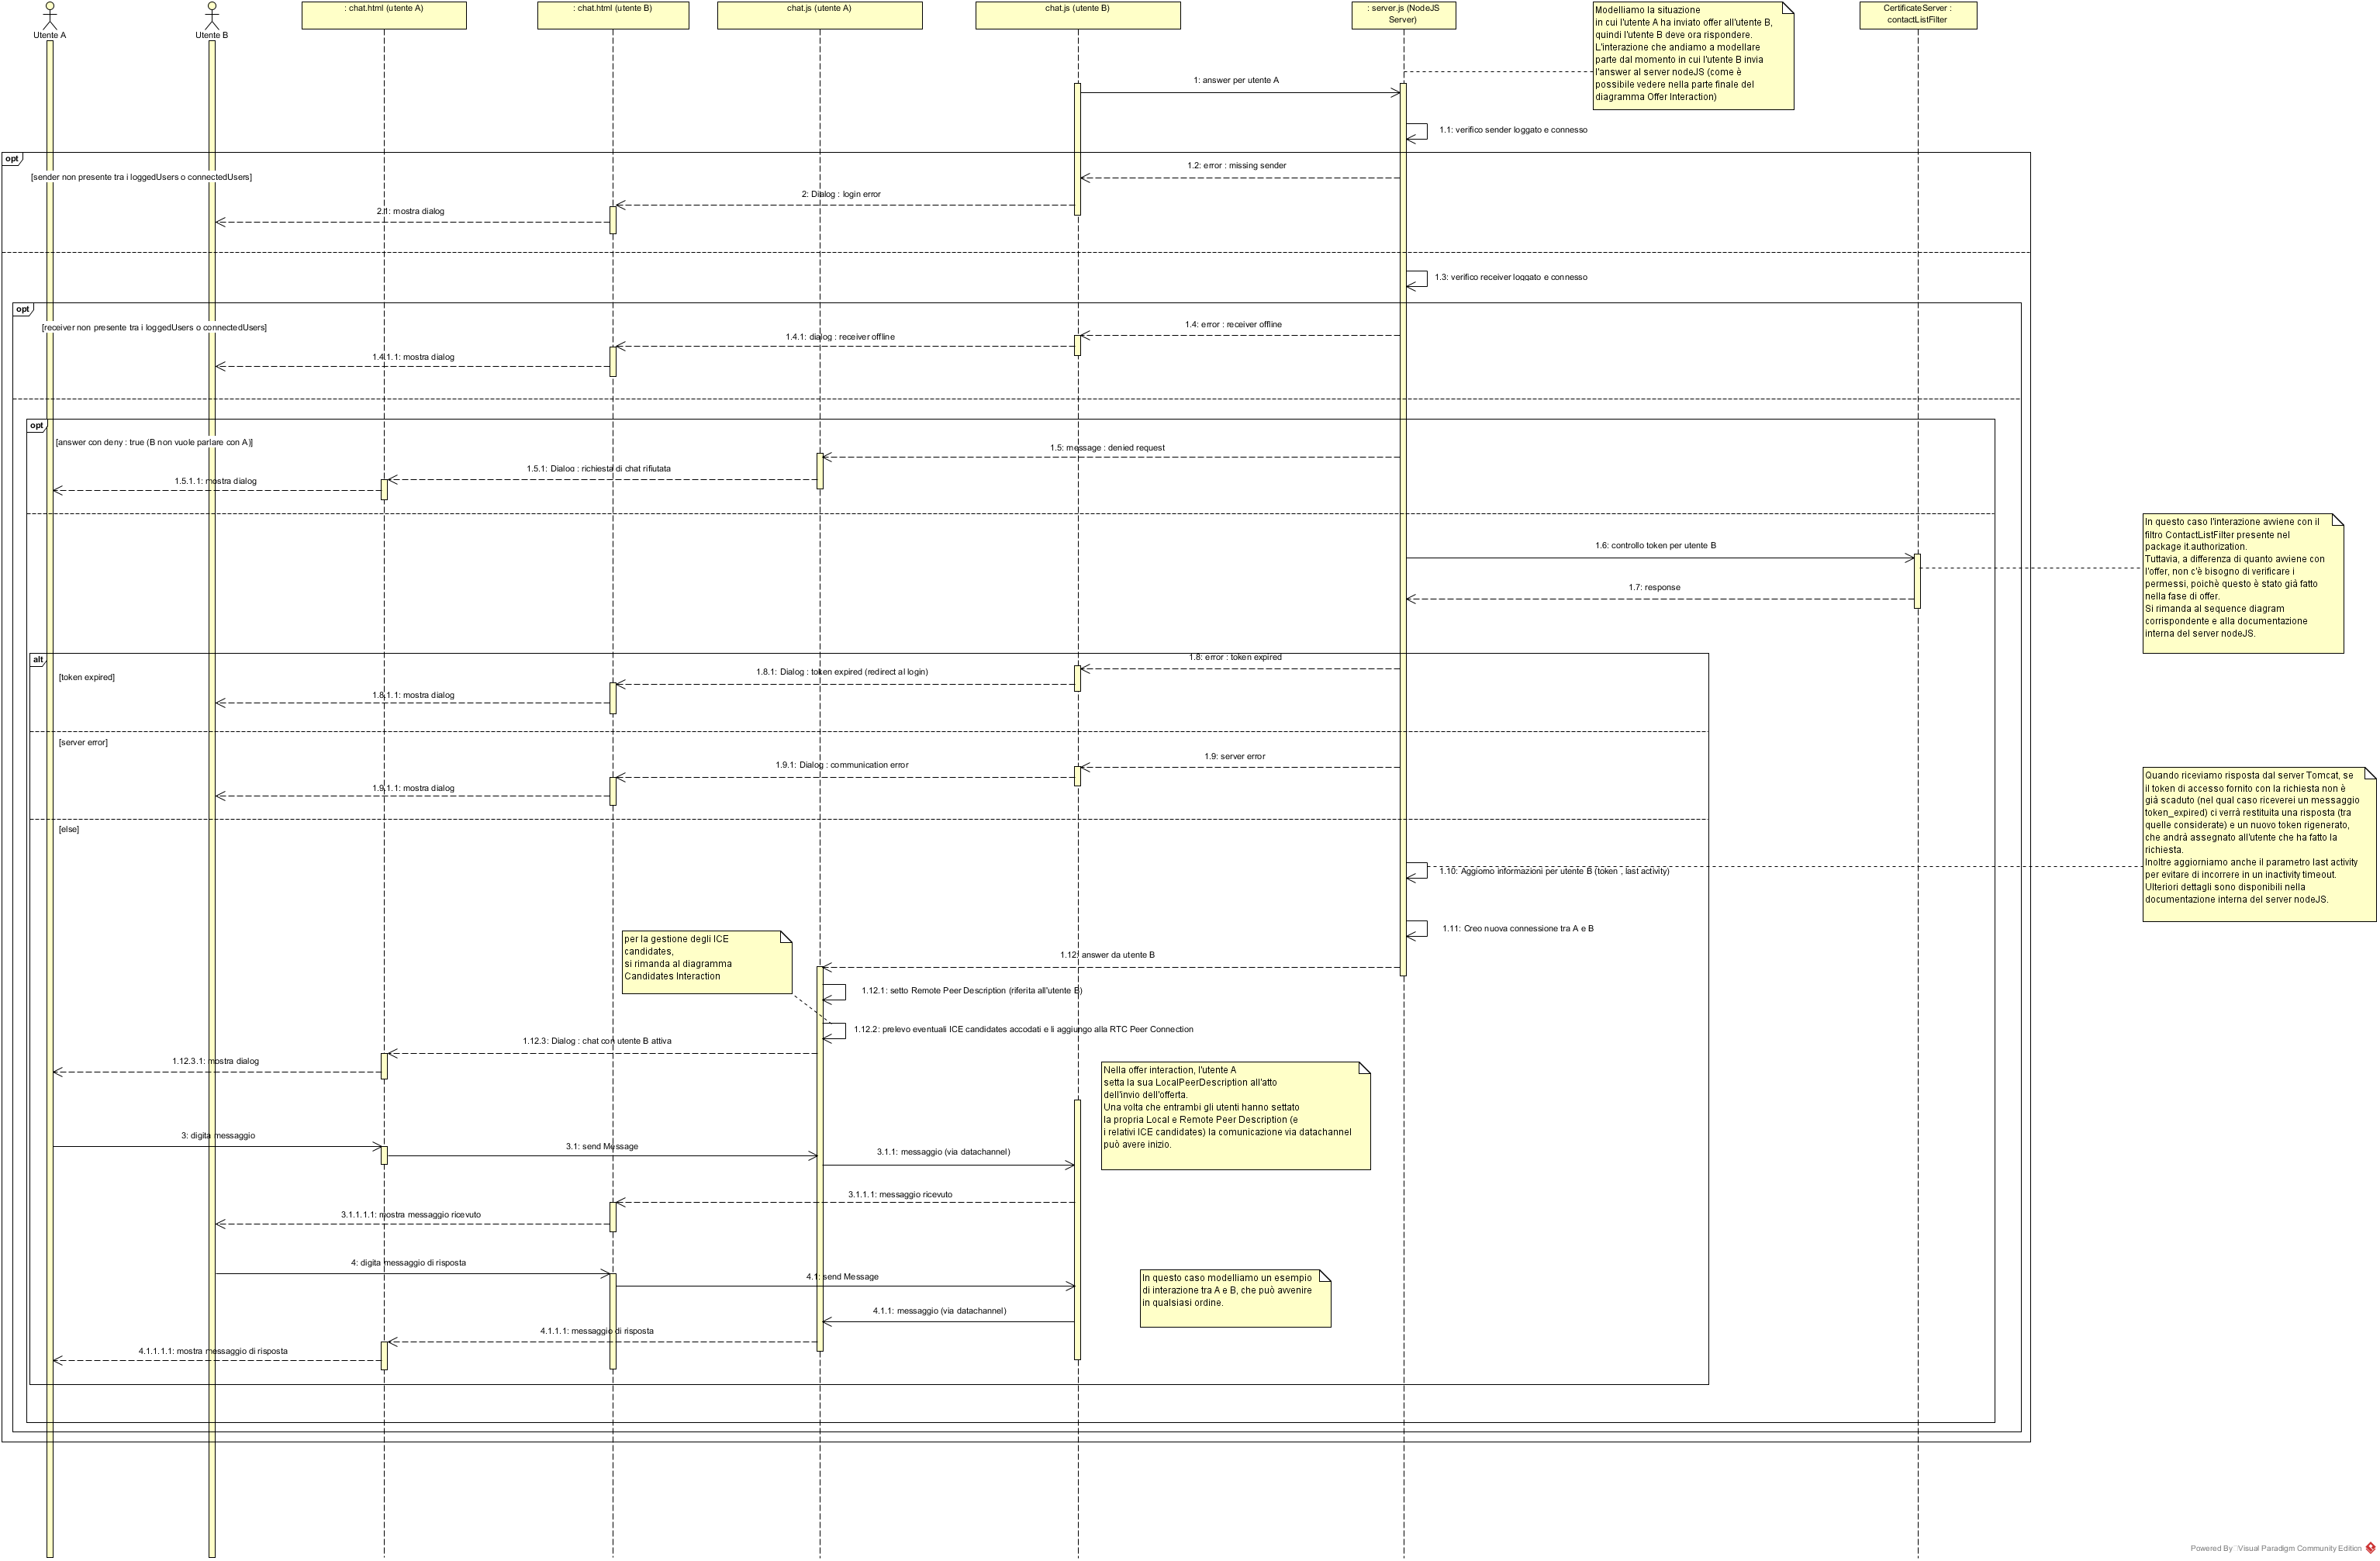
\includegraphics[scale = .26]{img/sequence_answer.png}
	\caption{Answer Interaction}
	\label{gfx:answerinteraction}
\end{figure}
\end{center}	
\end{landscape}%
Si nota che, in tal caso, quando l'utente B riceve l'offer da parte dell'utente A, si possono verificare due situazioni:
\begin{itemize}
\item l'utente B \textit{rifiuta} di parlare con l'utente A;
\item l'utente B \textit{accetta} di parlare con l'utente A.
\end{itemize}

Nel primo caso, l'utente B invierà al signaling server un messaggio answer contenente un campo \textit{deny}, con il quale il server nodeJS capirà che l'utente B ha rifiutato la chiamata e potrà quindi avvertire l'utente A di tale situazione.\\
Nel secondo caso, il server nodeJS riceverà un messaggio answer da parte dell'utente B, che dovrà poi essere recapitato ad A dopo aver verificato le stesse condizioni di prima.\\
In particolare, il server nodeJS si occuperà di:
\begin{itemize}
\item verificare che l'utente A sia loggato e connesso (ovvero: presente tra loggedUsers e connectedUsers)
\item verificare che l'utente B sia loggato e connesso (ovvero: presente tra loggedUsers e connectedUsers)
\item verificare che l'access token di B sia valido
\item verificare che l'utente B non abbia rifiutato di rispondere (in altri termini: se A chiama B, B può decidere di non rispondere)
\item verificare che A abbia il permesso di parlare con B (contattando il server tomcat e usando policy XACML)
\end{itemize}

Nel caso in cui una di queste condizioni non dovesse essere verificata, l'utente B (ed eventualmente l'utente A) saranno opportunamente avvertiti mediante appositi messaggi di stato.\\
Se invece la procedura va a buon fine, il signaling server si occuperà di inoltrare il messaggio di answer verso l'utente A: questo consentirà all'utente A di configurare sia la propria \textit{LocalPeerDescription} (locale ad A) sia la \textit{RemotePeerDescription} (legata all'utente B e ottenuta con le informazioni contenute nella answer).\\
In questo modo (una volta avvenuta anche la configurazione degli ICE candidates) la connessione è finalmente stabilita, e quindi utente A e utente B possono iniziare lo scambio di messaggi.\\
Per ulteriori dettagli si rimanda alla documentazione interna del server nodeJS.\\

\subsection{ICE Candidates Interaction}

In figura \ref{gfx:candidatesinteraction}, il sequence diagram illustra il meccanismo con cui avviene la comunicazione e lo scambio degli ICE candidates tra l'utente A e l'utente B.

\begin{figure}[!htbp]
	\centering
	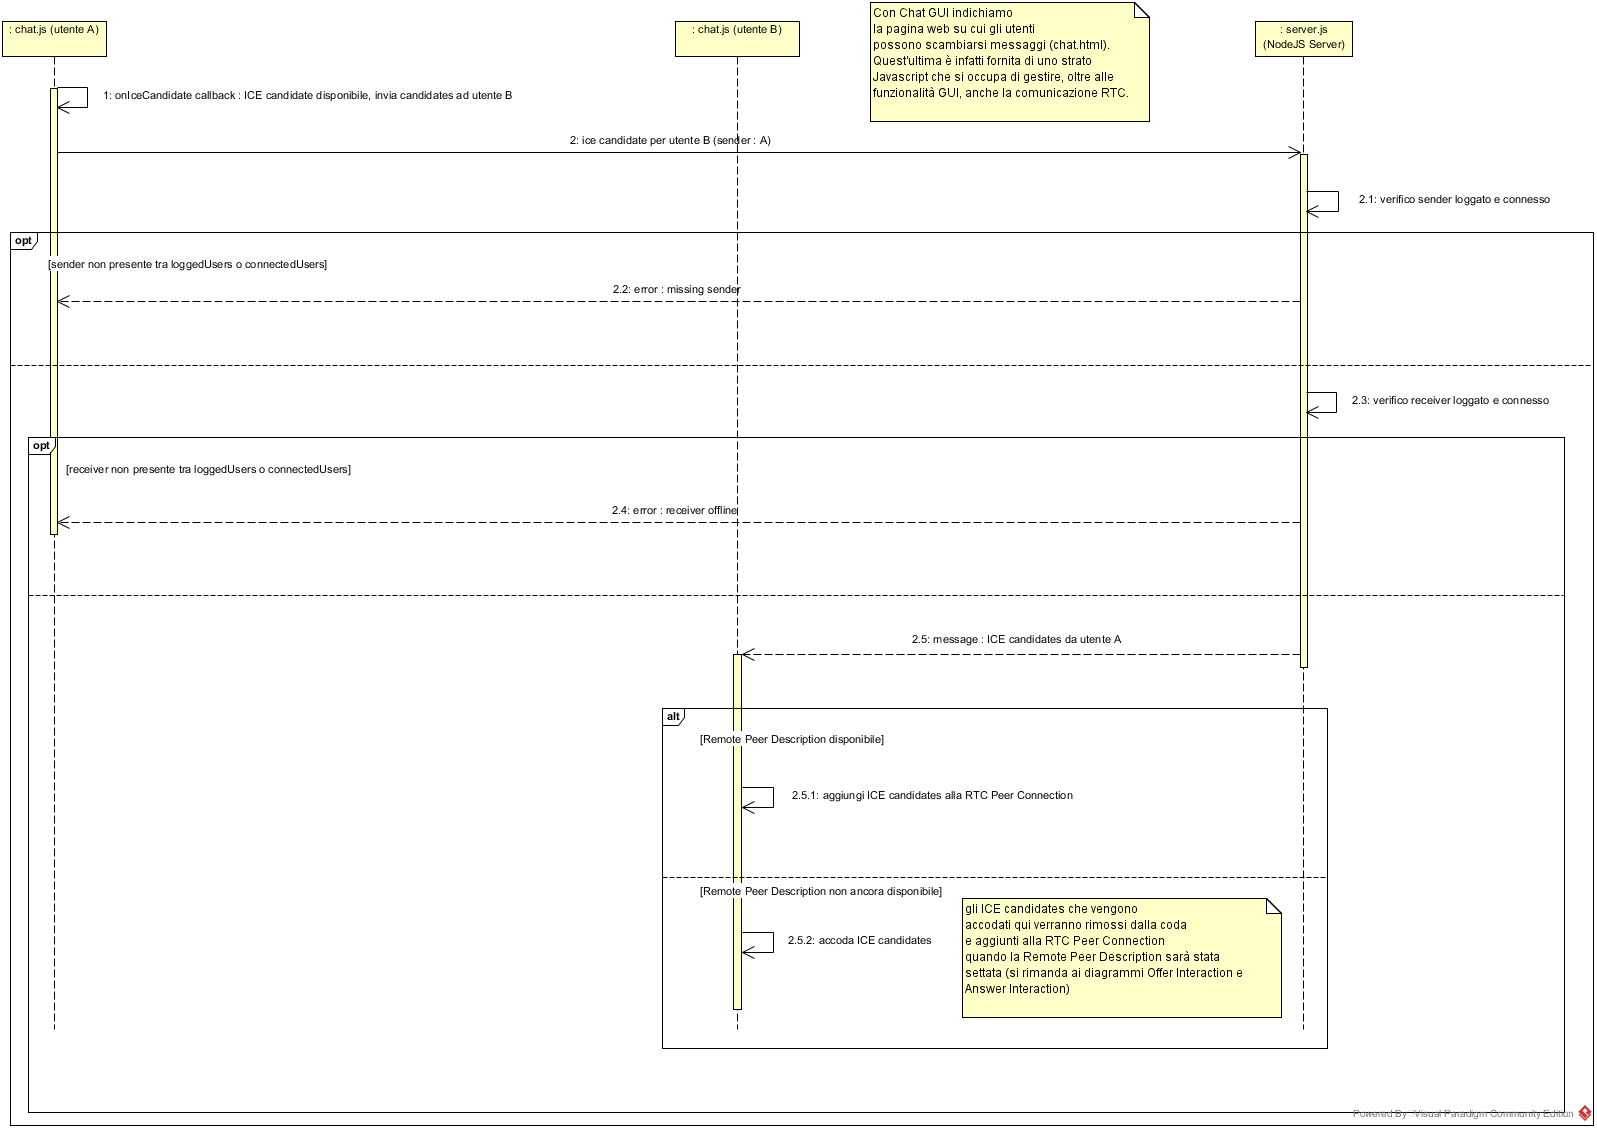
\includegraphics[scale = .37]{img/sequence_candidates.png}
	\caption{Candidates Interaction}
	\label{gfx:candidatesinteraction}
\end{figure}

Entrambi i client posseggono dei \textit{listener} per cui, non appena un ICE candidate risulta disponibile, viene inviato un messaggio verso il signaling server contenente informazioni a riguardo.\\
Il signaling server, dopo aver effettuato gli usuali controlli legati alla presenza degli utenti tra i \textit{loggedUsers} e i \textit{connectedUsers}, si occuperà semplicemente di inoltrare gli ICE candidates da un utente all'altro.\\
Tuttavia, visto che la configurazione degli ICE candidates può avvenire soltanto quando la RemotePeerDescription è stata settata, andremo ad accodare gli ICE candidates finchè non otterremo una RemotePeerDescription: a quel punto preleveremo i candidates dalla coda e configureremo di conseguenza la nostra connessione verso l'altro peer.\\
Ulteriori dettagli possono essere ottenuti osservando la documentazione interna del server nodeJS.\\

\subsubsection{Inactivity Timeout Interaction}

Il sequence diagram riportato di seguito mostra il meccanismo con cui è possibile rimuovere automaticamente un utente inattivo se quest'ultimo non effettua operazioni per più di un certo periodo di tempo.

\begin{figure}[!htpb]
	\centering
	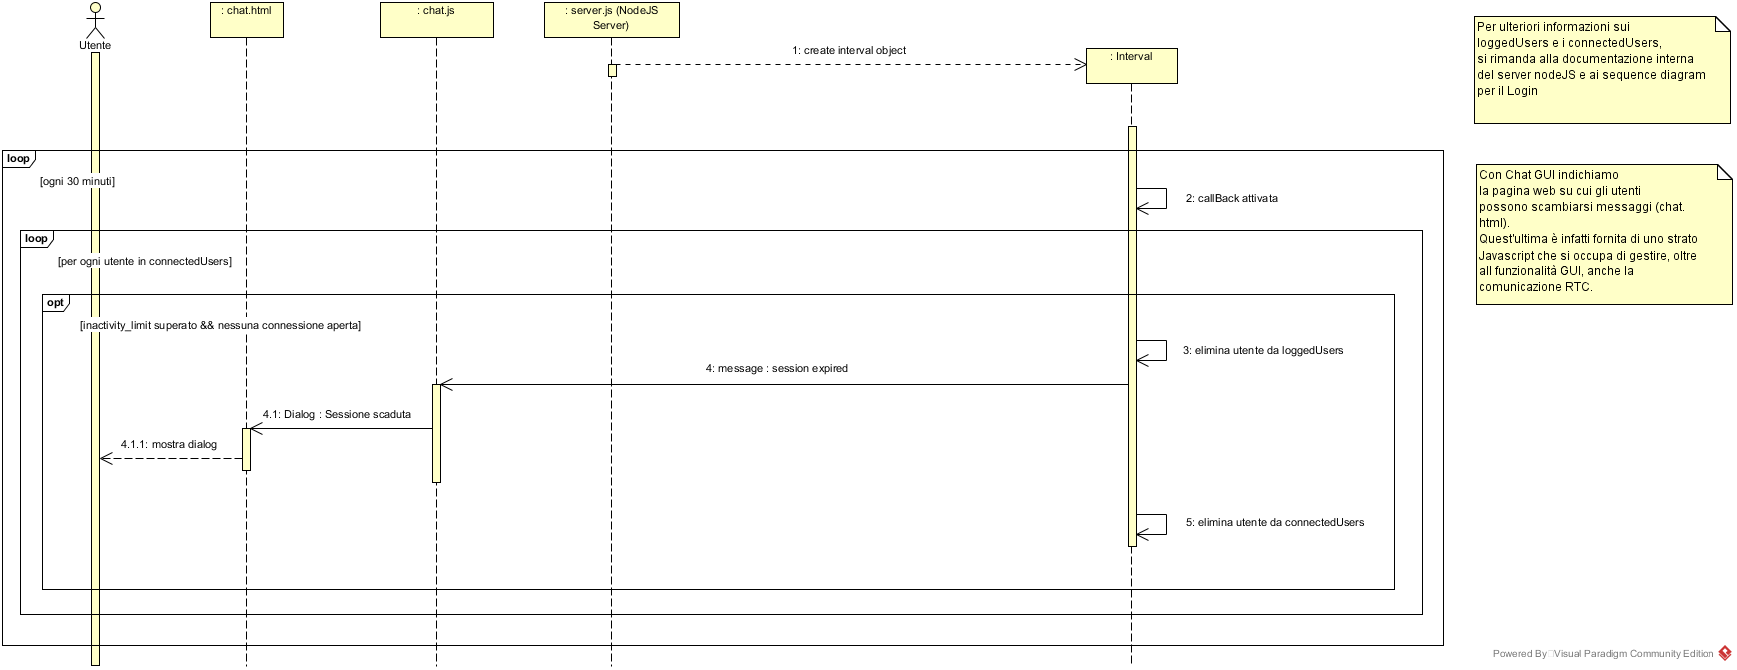
\includegraphics[scale = .35]{img/sequence_timeout.png}
	\caption{Timeout Inactivity Interaction}
	\label{gfx:timeoutinteraction}
\end{figure}

Il timeout è stato programmato per scattare ogni 5 minuti.\\
Quando la callback associata al timeout viene invocata, andremo ad analizzare tutti gli utenti con connessioni attive verso il signaling server (presenti tra i connectedUsers) per identificare quegli utenti che sono rimasti \textit{inattivi} (ovvero che non hanno inviato answer/offer e che non possiedono connessioni attive): tali utenti verranno quindi rimossi dai loggedUsers e dai connectedUsers, notificando l'evento con un apposito messaggio di stato lato client.\\

\subsection{Contact List Filter}

Il diagramma in figura \ref{gfx:contactlistfilter} mostra il comportamento del filtro ContactListFilter, utilizzato per l'accesso alle contact-lists che vengono prelevate dagli utenti ogni volta che si connettono alla chat, per poter selezionare (in base a policy ben precise) con quale utente comunicare.

\begin{figure}[!htbp]
		\centering
	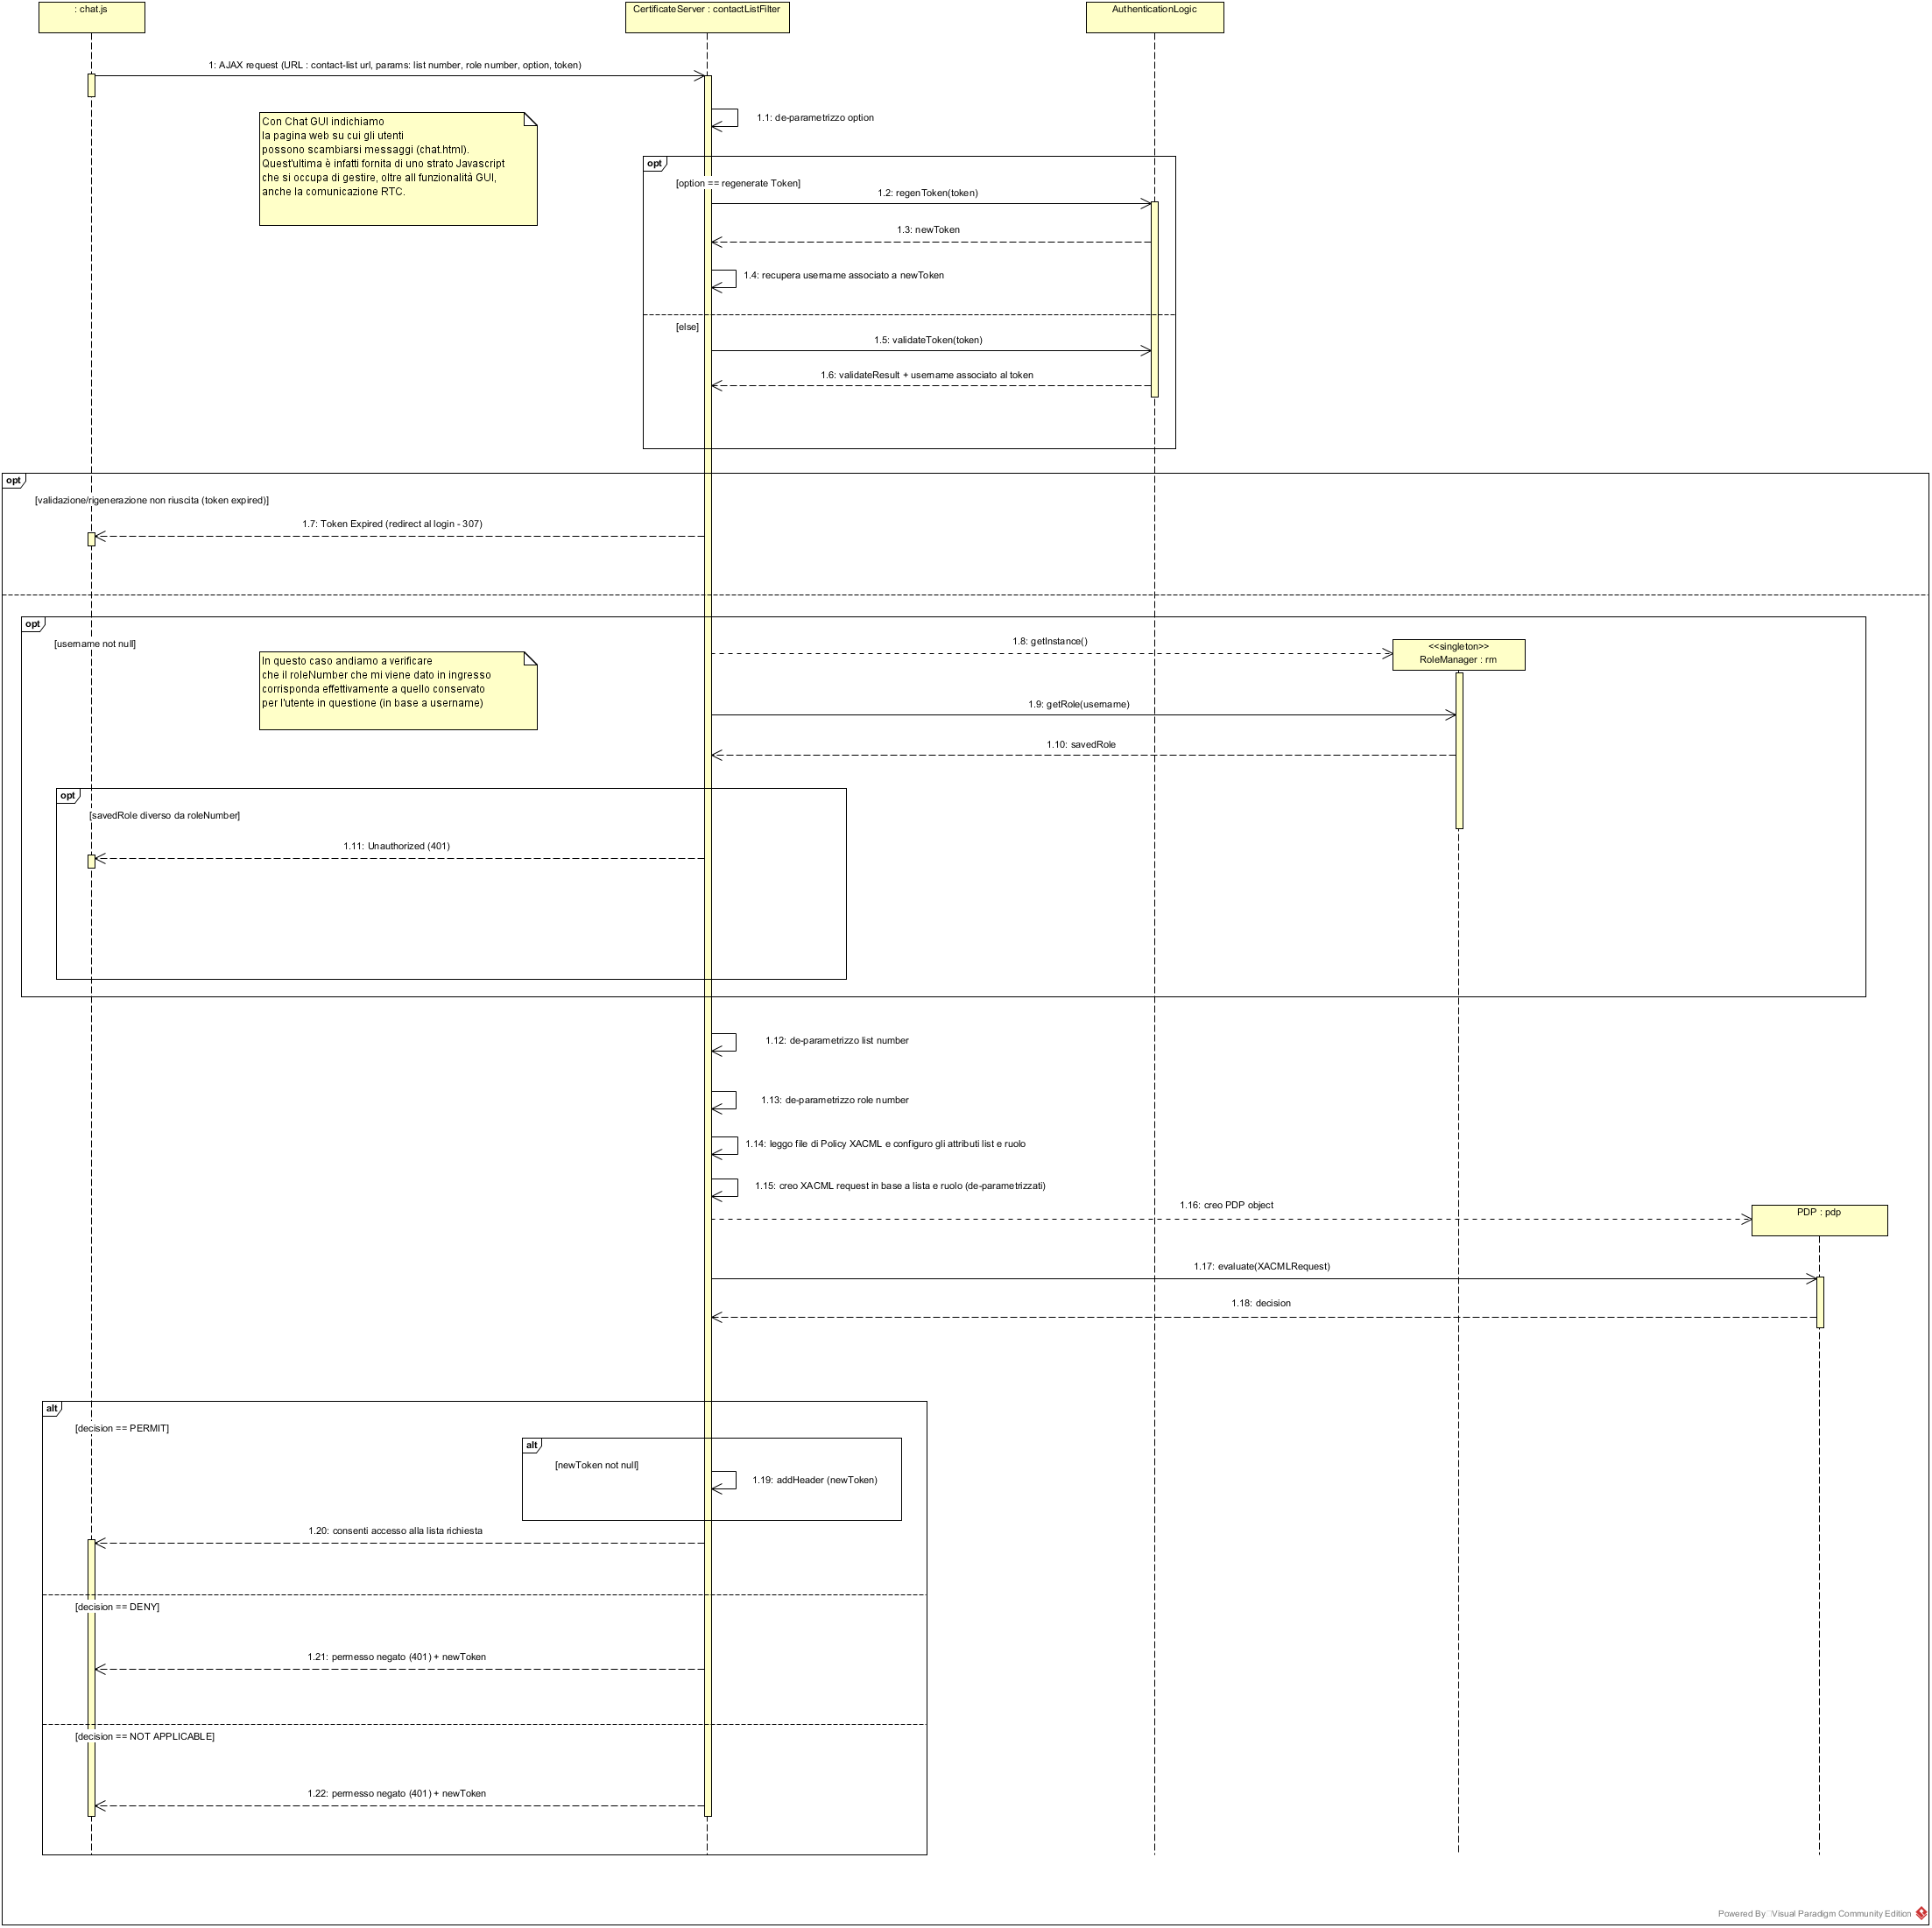
\includegraphics[scale = .26]{img/sequence_contactlist.png}
	\caption{Contact List Filter}
	\label{gfx:contactlistfilter}
\end{figure}
Il filtro viene attivato ogniqualvolta viene richiesto l'accesso al contenuto della cartella contact-lists, in accordo con quanto dichiarato nel file web.xml.\\
Le richieste contengono tipicamente i seguenti parametri (POST):
\begin{itemize}
\item list : lista a cui accedere
\item role : ruolo dell'utente richiedente
\item token: token di accesso
\item option : valore che indica rigenerazione/validazione del token
\end{itemize}
Alla ricezione della richiesta, verrà effettuata una de-parametrizzazione dei dati passati tramite POST (sfruttando una \textit{Integer Access Reference Map}, accessibile \href{https://static.javadoc.io/org.owasp.esapi/esapi/2.0.1/org/owasp/esapi/AccessReferenceMap.html}{qui}.\\
Dopodichè, andremo a verificare se è stata richiesta la rigenerazione del token o la sua semplice validazione: nel caso in cui il token dovesse essere scaduto, entrambe queste procedure falliranno: questo produrrà il sollevamento di un'eccezione con cui segnaleremo, lato client, un \textit{temporary redirect} (307) che reindirizzerà l'utente al login.\\
Una volta assicuratoci che il token di accesso è valido, andremo innanzitutto a verificare che il ruolo fornito dall'utente sia corrispondente al suo ruolo effettivo, dopodichè de-parametrizzeremo i dati che rappresentano lista e ruolo, per poi costruire la richiesta XACML che verrà sottoposta al PDP (\textit{Policy Decision Point}), previa lettura del file \textit{policy.xml} che contiene le XACML policies da applicare.\\
In caso di accesso consentito, il filtro si limita semplicemente ad allegare il token rinnovato (se presente) e a far avanzare correttamente la richiesta; in caso di permesso negato, invieremo comunque il token rinnovato (se presente), ma notificheremo il client con uno status code 401 (Unauthorized).\\

Per ulteriori dettagli, si rimanda alla documentazione interna del server nodeJS o del contact list filter.\\

